
\section{Introducción}
La Fase 1 del proyecto consiste en recolectar información real de un espacio seleccionado. En este caso, se trata de un lote donde se construirá una vivienda. No hay instalación eléctrica existente, por lo que el levantamiento se centra en dimensiones del terreno, áreas por nivel y distribución propuesta. Esto permitirá diseñar desde cero el sistema de iluminación en serie y paralelo según normativa RETIE.

\section{Objetivos de la Fase 1}
\subsection{Objetivo general}
Recolectar datos arquitectónicos del lote y de la vivienda proyectada para soportar el diseño eléctrico.

\subsection{Objetivos específicos}
\begin{itemize}
    \item Medir dimensiones del lote (largo, ancho, área total).
    \item Registrar áreas de construcción por nivel (planta baja, primer nivel, accesos, jardín).
    \item Identificar la distribución de espacios (sin construcción, se usan planos arquitectónicos).
    \item Elaborar croquis preliminar con medidas.
    \item Detectar necesidades de iluminación desde la etapa de diseño.
\end{itemize}

\section{Metodología de levantamiento}
Se realizó visita al lote ubicado en [dirección o referencia] el [fecha]. Se utilizó cinta métrica (precisión ±1 cm), cámara fotográfica y planos arquitectónicos proporcionados por el propietario. Actividades:
\begin{enumerate}
    \item Medición del lote: largo 20.00 m, ancho 10.00 m.
    \item Registro de áreas por nivel según planos:
        \begin{itemize}
            \item Planta baja: 95.00 m²
            \item Primer nivel: 123.06 m²
            \item Acceso / garaje / pasillo: 59.50 m²
            \item Jardín con barbacoa: 45.50 m²
            \item Total construcción: 277.56 m²
        \end{itemize}
    \item Toma de medidas de habitaciones (de planos): largo y ancho de cada ambiente (Tabla \ref{tab:medidas_habitaciones}).
    \item Croquis a mano alzada (Figura \ref{fig:croquis}).
    \item Registro fotográfico del lote (Figuras \ref{fig:foto1} a \ref{fig:foto3}).
    \item Identificación de necesidades: al no haber construcción, se diseñará iluminación con topología paralela para cada ambiente.
\end{enumerate}

\section{Resultados}

\subsection{Dimensiones del lote y construcción}
La Tabla \ref{tab:lot} resume las dimensiones del terreno y las áreas construidas por nivel.

\begin{table}[h]
\centering
\caption{Dimensiones del lote y áreas de construcción}
\label{tab:lot}
\begin{tabular}{|l|c|}
\hline
\textbf{Parámetro} & \textbf{Valor} \\
\hline
Largo del lote & 20.00 m \\
Ancho del lote & 10.00 m \\
Área total del lote & 200.00 m² \\
\hline
Planta baja & 95.00 m² \\
Primer nivel & 123.06 m² \\
Acceso / garaje / pasillo & 59.50 m² \\
Jardín con barbacoa & 45.50 m² \\
\textbf{Total construcción} & \textbf{277.56 m²} \\
\hline
\end{tabular}
\end{table}

\subsection{Medidas de habitaciones (desde planos)}
En la Tabla \ref{tab:medidas_habitaciones} se listan las dimensiones de los principales ambientes según los planos arquitectónicos.

\begin{table}[h]
\centering
\caption{Medidas de habitaciones (largo × ancho)}
\label{tab:medidas_habitaciones}
\begin{tabular}{|l|c|c|}
\hline
\textbf{Ambiente} & \textbf{Largo (m)} & \textbf{Ancho (m)} \\
\hline
Sala-comedor & 4.48 & 4.55 \\
Cocina & 3.50 & 2.00 \\
Habitación principal & 4.00 & 3.50 \\
Baño & 1.93 & 1.35 \\
Pasillo & 3.15 & 1.22 \\
Jardín & 6.50 & 7.00 \\
\hline
\end{tabular}
\end{table}
Nota: Las medidas se obtuvieron de los planos de diseño; pueden variar ligeramente en ejecución.

\subsection{Croquis preliminar}
La Figura \ref{fig:croquis} muestra el croquis a mano alzada con la distribución general del lote y ubicación de los volúmenes construidos.

\begin{figure}[h]
\centering
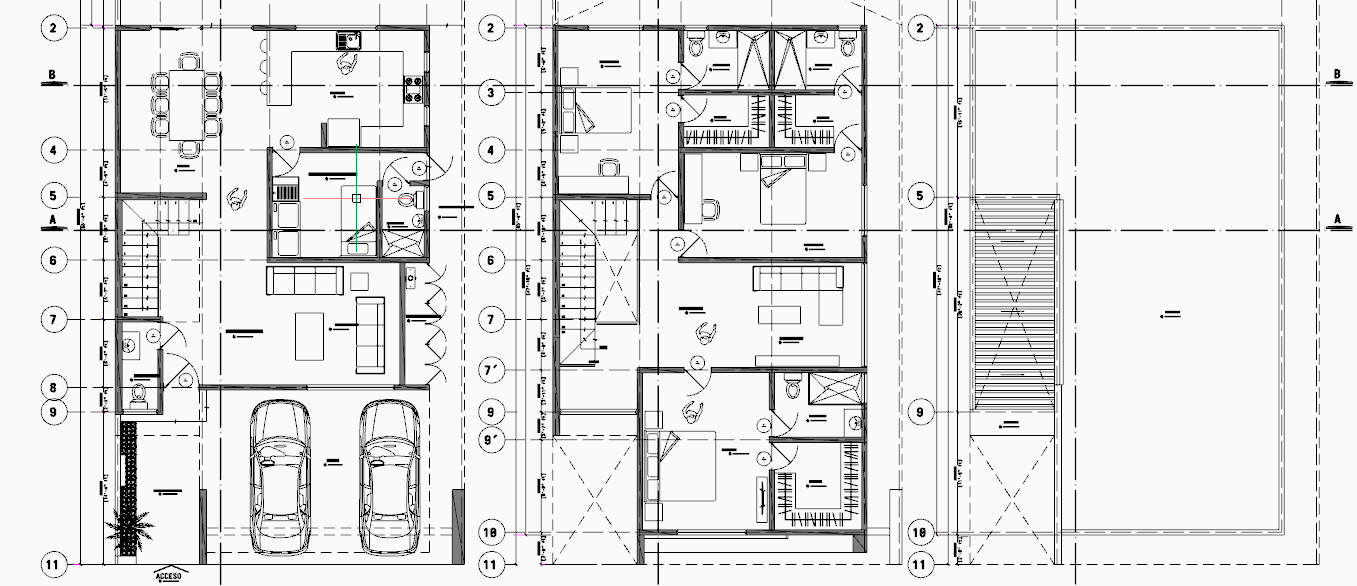
\includegraphics[width=0.6\linewidth]{croquis.png}
\caption{Croquis del lote y distribución de niveles.}
\label{fig:croquis}
\end{figure}

\subsection{Registro fotográfico}
Las Figuras \ref{fig:foto1} a \ref{fig:foto3} documentan el estado actual del lote (terreno sin construir).

\begin{figure}[h]
\centering
\includegraphics[width=0.6\linewidth]{foto_lugar.jpg}
\caption{Vista general del lote.}
\label{fig:foto1}
\end{figure}

\begin{figure}[h]
\centering
\includegraphics[width=0.6\linewidth]{foto_luminaria.jpg}
\caption{No existen luminarias por ser terreno sin construir.}
\label{fig:foto2}
\end{figure}

\begin{figure}[h]
\centering
\includegraphics[width=0.6\linewidth]{foto_interruptor.jpg}
\caption{No existe cableado ni interruptores.}
\label{fig:foto3}
\end{figure}

\subsection{Identificación de problemas y mejoras}
Al no haber construcción, los problemas se refieren al diseño futuro:
\begin{itemize}
    \item \textbf{Problema potencial}: Uso de conexión serie en iluminación causaría caída de tensión y dependencia de lámparas.
    \item \textbf{Mejora propuesta}: Diseñar circuitos independientes en paralelo para cada ambiente, con interruptores individuales.
    \item \textbf{Oportunidad}: Instalar cableado de calibre adecuado (\#14 AWG) y tubería conduit desde la construcción inicial.
    \item \textbf{Necesidad de simulación}: Validar el comportamiento de ambos tipos de conexión antes de la instalación real.
\end{itemize}

\section{Conclusiones de la Fase 1}
\begin{itemize}
    \item Se completó el levantamiento del lote y las áreas de construcción (total 277.56 m²).
    \item Se obtuvieron medidas precisas de los ambientes desde los planos arquitectónicos.
    \item Al no existir sistema de iluminación previo, el diseño partirá de cero, lo que permite aplicar la topología paralela desde el inicio.
    \item El croquis y las fotos (pendientes de tomar) servirán como evidencia del trabajo de campo.
    \item La Fase 2 utilizará estos datos para generar planos arquitectónico y eléctrico, y los cálculos correspondientes.
\end{itemize}

